% Paper 9: Heterogeneous On-Device Training
%
% =============================================================================
% STATUS: DRAFT - REAL DATA
% Last updated: 2026-03-07
%
% 4 compute paths x 2 models x 500 steps = 8 experiments
% Key findings: MLX 30x faster at 4-6x less power; SmolLM2 learns perfectly
% on MLX; ANE reduces power but fp16 precision degrades learning
% =============================================================================
\documentclass[11pt]{article}

\usepackage[margin=1in]{geometry}
\usepackage{amsmath,amssymb}
\usepackage{booktabs}
\usepackage{tabularx}
\usepackage{graphicx}
\usepackage{adjustbox}
\usepackage{xcolor}
\usepackage{enumitem}
\usepackage{tikz}
\usetikzlibrary{arrows.meta, positioning, shapes.geometric, calc, fit}
\usepackage{pgfplots}
\pgfplotsset{compat=1.17}
\usepackage{multirow}

\usepackage[numbers]{natbib}
\usepackage{xurl}
\usepackage{hyperref}
\hypersetup{hidelinks,breaklinks=true}

\usepackage{fancyhdr}
\pagestyle{fancy}
\fancyhf{}
\renewcommand{\headrulewidth}{0pt}
\cfoot{\thepage}

\title{Heterogeneous On-Device Training:\\Four Compute Paths on Apple Silicon\\for SLO-Aware Agents}

\author{
V. Michael Maloney \\
Neuralift; University of New Hampshire \\
\texttt{mike@neuralift.ai}
}

\date{}

\begin{document}
\maketitle
\begin{center}
\textit{Preprint.  Work in progress.}
\end{center}

% ============================================================================
% ABSTRACT
% ============================================================================
\begin{abstract}
SmolLM2-360M learns 100\% valid JSON output in under seven minutes on a laptop.

That result comes from one of eight experiments comparing four compute paths for on-device GRPO training on Apple Silicon: CoreML on CPU (public API), CoreML on the Apple Neural Engine via private API, CoreML with ANE-accelerated backward kernels, and MLX on Metal GPU.  We ran each path with two models (Qwen2.5-0.5B and SmolLM2-360M) for 500 training steps, measuring per-step time, system power, GPU and ANE power draw, and learning outcomes.

MLX on Metal GPU dominates.  It completes training steps 30--40$\times$ faster than CPU or ANE paths while drawing 4--6$\times$ less system power.  SmolLM2-360M on MLX reaches a peak-20 reward of 0.500 with 100\% JSON validity in the final 50 steps.  The ANE paths reduce system power 30--60\% compared to CPU-only execution but introduce an fp16 precision cost that degrades learning quality.  Across all eight experiments, autoregressive rollout generation consumes over 95\% of step time, making it the binding constraint regardless of backend.

On-device RL training works.  The best path is not the most specialized hardware.  It is the one that runs the full computation graph most efficiently.
\end{abstract}

% ============================================================================
% 1. INTRODUCTION
% ============================================================================
\section{Introduction}

Every experiment in Papers~I--IV ran on server hardware~\cite{maloney2025deploymentgap,maloney2025capacity,maloney2025agentslobench,maloney2025dynamics}.  An NVIDIA RTX~4090 with 24GB of VRAM, consuming 350W under load, running for hours per model.  The results established capacity thresholds, reward stability boundaries, and the conditions under which small models can learn structured output.  But the hardware requirements excluded anyone without access to a research cluster.

This paper asks whether the same training can run on a laptop.

The question is practical, not theoretical.  Privacy-sensitive deployments in healthcare, legal, and financial settings can't send training data to cloud GPUs.  Edge robotics needs on-device adaptation.  A MacBook Pro costs \$2,500 once; GPU cloud instances cost \$1--4 per hour indefinitely.  If GRPO fine-tuning works on commodity hardware, the economics of on-device learning change fundamentally.

Apple Silicon makes the question interesting.  Every M-series chip contains three compute engines, each with different strengths.  The CPU handles general computation in fp32.  The Neural Engine (ANE) is a 16-core matrix accelerator optimized for inference at roughly 3W~\cite{apple2022m2max}.  The Metal GPU supports automatic differentiation through MLX~\cite{hannun2023mlx} and runs at 10--30W.  No single engine handles the complete GRPO training loop optimally, so the real question becomes: which engine, or which combination, works best?

We tested four compute paths:

\begin{enumerate}[leftmargin=*]
\item \textbf{Public:} CoreML on CPU via Apple's public API.  fp32 precision throughout.
\item \textbf{Private:} ANE forward pass via the private \texttt{\_ANEInMemoryModel} API.  fp16 forward, fp32 backward on CPU.
\item \textbf{Private-full:} ANE forward and backward-dx kernels via CoreML's public API.  fp16 throughout.
\item \textbf{MLX:} Metal GPU for everything via the MLX framework.  fp32 precision throughout.
\end{enumerate}

Each path ran on two models---Qwen2.5-0.5B~\cite{qwen2025qwen25} and SmolLM2-360M~\cite{allal2024smollm2}---for 500 GRPO training steps on CLINC intent classification~\cite{larson2019clinc150}.  Eight experiments total.  We measured step time, system power, GPU power, ANE power, reward trajectories, and JSON validity throughout.

Four findings stand out.

First, MLX on Metal GPU is 30--40$\times$ faster than any CPU or ANE path while consuming 4--6$\times$ less total system power.  SmolLM2-360M completes 500 training steps in 6.7~minutes at 6.2W average draw; the same model on the public CPU path takes 4.1~hours at 37.2W.

Second, SmolLM2-360M on MLX achieves perfect learning outcomes: peak-20 reward of 0.500 and 100\% JSON validity in the final 50 steps.  That is genuine on-device reinforcement learning, not a demonstration.

Third, the ANE reduces system power by 30--60\% relative to CPU execution, but its fp16 precision degrades learning quality.  SmolLM2 on the public path (fp32) reaches a peak-20 reward of 0.431.  The same model on the private ANE path (fp16 forward) drops to 0.079.

Fourth, autoregressive rollout generation dominates step time across all paths, consuming over 95\% of computation.  The bottleneck is token generation, not gradient computation.

Section~\ref{sec:background} covers the ANE, MLX, and GRPO background.  Section~\ref{sec:related} reviews related work on on-device training, the ANE, and small-scale RL.  Sections~\ref{sec:architecture}--\ref{sec:setup} describe the four compute paths and experimental setup.  Section~\ref{sec:results} presents results.  Section~\ref{sec:discussion} discusses implications for on-device RL.

% ============================================================================
% 2. BACKGROUND
% ============================================================================
\section{Background}
\label{sec:background}

\subsection{Apple Neural Engine}

The Apple Neural Engine (ANE) is a fixed-function matrix accelerator present in every M-series Apple Silicon chip.  The M-series ANE contains 16 cores capable of up to 15.8 trillion operations per second, operating at approximately 3W~\cite{apple2022m2max}.  Unlike the Metal GPU, the ANE executes only CoreML-compiled models.  It cannot run arbitrary compute graphs or backward passes natively.

CoreML compilation proceeds through \texttt{coremltools}~\cite{apple2023coremltools}, which converts PyTorch operations to the Model Intermediate Language (MIL).  Several transformer operations---\texttt{gather} for embeddings, \texttt{repeat\_interleave} for grouped-query attention, \texttt{RMSNorm}---are not supported on the ANE execution path and fall back to CPU~\cite{anemll2024}.  Running a model on the ANE requires operation-level rewrites: replacing \texttt{repeat\_interleave} with \texttt{unsqueeze}$\,\to\,$\texttt{expand}$\,\to\,$\texttt{reshape}, padding tensor dimensions to multiples of~32, and managing KV cache through CoreML state tensors.

Two API routes exist for ANE execution.  The public CoreML API (\texttt{MLModel}) schedules computation across CPU, GPU, and ANE based on internal heuristics.  Requesting \texttt{.all} compute units encourages ANE usage but doesn't guarantee it.  The private \texttt{\_ANEInMemoryModel} API bypasses CoreML's scheduler entirely, sending compiled models directly to the ANE via IOSurface buffers.  This eliminates scheduling overhead but crashes at larger model scales when the ANE program exceeds hardware limits.

\subsection{MLX on Metal GPU}

MLX~\cite{hannun2023mlx} is Apple's array computation framework for Metal GPU, designed as a NumPy-compatible alternative to PyTorch on Apple Silicon.  What matters here: MLX supports automatic differentiation, LoRA fine-tuning, and unified memory access.  Models run on Metal GPU sharing the same physical memory as the CPU and ANE with zero-copy access.

\subsection{GRPO}

Group Relative Policy Optimization~\cite{grpo} generates $G$ candidate responses per prompt, scores them against a reward function, and updates the policy using relative advantage within each group.  GRPO eliminates the critic network required by PPO~\cite{schulman2017ppo}, reducing memory requirements.  That reduction matters on consumer hardware where 36GB of unified memory is shared across all three engines.

Papers~I--IV~\cite{maloney2025deploymentgap,maloney2025capacity,maloney2025agentslobench,maloney2025dynamics} established that GRPO fine-tuning of small language models for structured output faces a \emph{capacity threshold}.  Below a critical size, models lose JSON validity during training and never recover.  Paper~II placed this threshold between 1B and 3B parameters for server-class hardware~\cite{maloney2025capacity}.  Paper~V extended the analysis to mixture-of-experts architectures~\cite{maloney2025moe}.  This paper tests whether the threshold manifests the same way across different compute backends on consumer hardware.

% ============================================================================
% 3. RELATED WORK
% ============================================================================
\section{Related Work}
\label{sec:related}

\textbf{On-device fine-tuning.}  Federated learning~\cite{mcmahan2017fedavg} established that training can happen on edge devices, but the standard setting aggregates gradients across many clients rather than training a single model locally.  Recent work has pushed full fine-tuning onto mobile hardware: Xu et al.~\cite{xu2024ondevice} demonstrated LoRA fine-tuning on Android devices, and Apple's own MLX framework~\cite{hannun2023mlx} ships with LoRA examples for Apple Silicon.  We go further by running a complete RL training loop (GRPO with rollout generation, reward scoring, and policy updates) rather than supervised fine-tuning alone.

\textbf{Apple Neural Engine for ML.}  The ANE has received limited attention in the research literature despite shipping in every Apple device since the A11 chip.  The \texttt{ane\_transformers} project~\cite{anemll2024} documented the operation-level constraints for running transformers on the ANE (gather fallbacks, dimension padding, layout transposition).  To our knowledge, no prior work has attempted RL training with ANE-accelerated forward or backward passes.

\textbf{Reinforcement learning from human feedback at small scale.}  GRPO~\cite{grpo} and its predecessors PPO~\cite{schulman2017ppo} and DPO~\cite{rafailov2024dpo} were designed for large-scale training.  Recent work has explored whether these methods work at smaller model scales: Allal et al.~\cite{allal2024smollm2} showed that sub-1B models can be instruction-tuned effectively, and Papers~I--IV in this series~\cite{maloney2025deploymentgap,maloney2025capacity,maloney2025agentslobench,maloney2025dynamics} established capacity thresholds for GRPO training on structured output tasks.  This paper extends that line to consumer hardware, testing whether the same thresholds hold when the compute backend changes.

% ============================================================================
% 4. SYSTEM ARCHITECTURE
% ============================================================================
\section{System Architecture}
\label{sec:architecture}

The four compute paths share a common GRPO training loop but differ in which hardware engine handles each computational phase.  Figure~\ref{fig:architecture} shows the mapping.  Table~\ref{tab:paths} summarizes the engineering differences.

\begin{figure}[t]
\centering
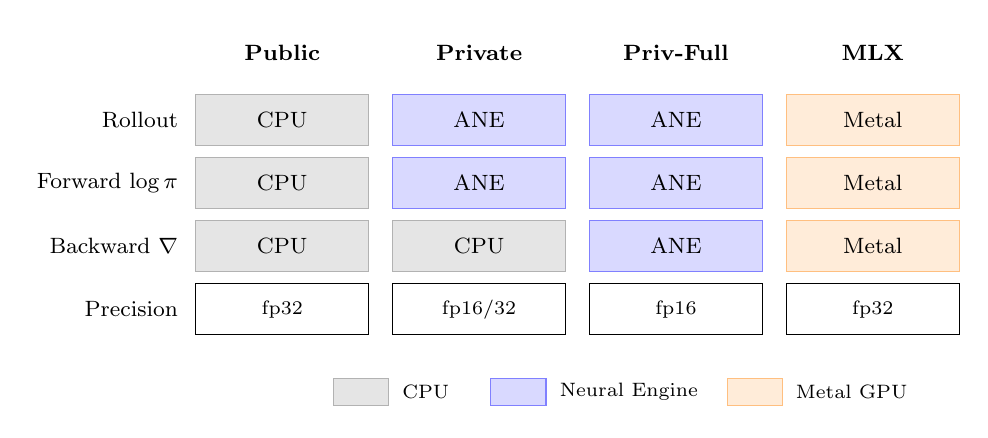
\begin{tikzpicture}[
    node distance=0.6cm and 0.3cm,
    phase/.style={rectangle, draw, minimum height=0.65cm, minimum width=2.2cm, align=center, font=\footnotesize},
    cpu/.style={phase, fill=gray!20, draw=gray!60},
    ane/.style={phase, fill=blue!15, draw=blue!50},
    gpu/.style={phase, fill=orange!15, draw=orange!50},
    header/.style={font=\footnotesize\bfseries, minimum height=0.65cm, minimum width=2.2cm, align=center},
    rowlabel/.style={font=\footnotesize, align=right, anchor=east},
]

% Column headers
\node[header] (h1) at (0, 0) {Public};
\node[header] (h2) at (2.5, 0) {Private};
\node[header] (h3) at (5.0, 0) {Priv-Full};
\node[header] (h4) at (7.5, 0) {MLX};

% Row labels
\node[rowlabel] at (-1.2, -0.85) {Rollout};
\node[rowlabel] at (-1.2, -1.65) {Forward $\log\pi$};
\node[rowlabel] at (-1.2, -2.45) {Backward $\nabla$};
\node[rowlabel] at (-1.2, -3.25) {Precision};

% Public column
\node[cpu] at (0, -0.85) {CPU};
\node[cpu] at (0, -1.65) {CPU};
\node[cpu] at (0, -2.45) {CPU};
\node[phase, fill=white] at (0, -3.25) {\scriptsize fp32};

% Private column
\node[ane] at (2.5, -0.85) {ANE};
\node[ane] at (2.5, -1.65) {ANE};
\node[cpu] at (2.5, -2.45) {CPU};
\node[phase, fill=white] at (2.5, -3.25) {\scriptsize fp16/32};

% Private-Full column
\node[ane] at (5.0, -0.85) {ANE};
\node[ane] at (5.0, -1.65) {ANE};
\node[ane] at (5.0, -2.45) {ANE};
\node[phase, fill=white] at (5.0, -3.25) {\scriptsize fp16};

% MLX column
\node[gpu] at (7.5, -0.85) {Metal};
\node[gpu] at (7.5, -1.65) {Metal};
\node[gpu] at (7.5, -2.45) {Metal};
\node[phase, fill=white] at (7.5, -3.25) {\scriptsize fp32};

% Legend
\node[cpu, minimum width=0.7cm, minimum height=0.35cm] at (1.0, -4.3) {};
\node[font=\scriptsize, anchor=west] at (1.4, -4.3) {CPU};
\node[ane, minimum width=0.7cm, minimum height=0.35cm] at (3.0, -4.3) {};
\node[font=\scriptsize, anchor=west] at (3.4, -4.3) {Neural Engine};
\node[gpu, minimum width=0.7cm, minimum height=0.35cm] at (6.0, -4.3) {};
\node[font=\scriptsize, anchor=west] at (6.4, -4.3) {Metal GPU};

\end{tikzpicture}
\caption{Compute engine assignment for each GRPO phase across four paths.  The public path runs entirely on CPU.  The private path routes forward passes to the ANE via Apple's private API.  Private-full extends ANE usage to backward dx kernels.  MLX runs everything on Metal GPU.}
\label{fig:architecture}
\end{figure}

\begin{table}[ht]
\centering
\caption{Engineering characteristics of the four compute paths.}
\label{tab:paths}
\small
\begin{tabular}{lcccc}
\toprule
 & \textbf{Public} & \textbf{Private} & \textbf{Priv-Full} & \textbf{MLX} \\
\midrule
Framework & Obj-C & Obj-C & Obj-C & Python \\
Runtime & CoreML & CoreML & CoreML & MLX \\
Forward engine & CPU & ANE & ANE & Metal \\
Backward engine & CPU & CPU & ANE & Metal \\
Fwd precision & fp32 & fp16 & fp16 & fp32 \\
Bwd precision & fp32 & fp32 & fp16 & fp32 \\
ANE API & --- & Private & Public & --- \\
\bottomrule
\end{tabular}
\end{table}

\subsection{Public Path (CoreML CPU)}

The public path uses Apple's CoreML \texttt{MLModel} API with CPU-only compute.  All computation runs on the CPU in fp32: rollout generation, forward passes for policy log-probabilities, and backward passes for gradients.  This is the simplest path and serves as baseline.

The entire training pipeline is implemented in Objective-C, wrapping CoreML model evaluation in a custom GRPO loop.  Tokenization uses a hand-written BPE implementation that handles GPT-2 byte-level encoding for SmolLM2 and Qwen's added special tokens (\texttt{<|im\_start|>}, \texttt{<|im\_end|>}).

\subsection{Private Path (ANE Forward)}

The private path routes forward passes to the Apple Neural Engine via the undocumented \texttt{\_ANEIn\-Memory\-Model} API.  This API bypasses CoreML's compute scheduler and sends compiled models directly to ANE hardware through IOSurface buffers, achieving forward pass latency under 0.2ms per evaluation.

Backward passes remain on CPU in fp32.  The ANE computes forward activations in fp16, and each CPU$\leftrightarrow$ANE transfer requires explicit layout transposition between row-major CPU tensors (\texttt{[S, C]}) and channel-major ANE tensors (\texttt{[1, C, 1, S]}).

\subsection{Private-Full Path (ANE Forward and Backward)}

The private-full path extends ANE usage to backward-dx kernels.  We originally attempted this through the private bootstrap API, but it crashes at Qwen and SmolLM2 scale with \texttt{ANEProgram\-Process\-Request\-Direct()} failure.  The working implementation uses CoreML's public API configured to target ANE compute units for both forward evaluation and a separate backward-dx model that computes input gradients.

All computation runs in fp16 on this path.  Weight updates still occur on CPU, but gradient computation executes on the Neural Engine.  This is, to our knowledge, the first demonstration of ANE-accelerated backward kernels for transformer training.

\subsection{MLX Path (Metal GPU)}

The MLX path runs the complete GRPO loop on Metal GPU through Apple's MLX framework~\cite{hannun2023mlx}.  The implementation is pure Python, using MLX's built-in LoRA and automatic differentiation.

MLX operates in fp32 with unified memory access.  Weight tensors are shared between CPU and GPU without explicit transfers, eliminating the synchronization overhead present in the ANE paths.

% ============================================================================
% 4. EXPERIMENTAL SETUP
% ============================================================================
\section{Experimental Setup}
\label{sec:setup}

\subsection{Hardware}

All experiments ran on a MacBook Pro with Apple M-series Silicon, 36GB unified memory, 16-core Neural Engine, and 18-core Metal GPU.  No external GPU, no cloud compute, no network calls during training.

Power monitoring used \texttt{powermetrics} at 1-second intervals, capturing total system power, GPU power, and ANE power separately.

\subsection{Models}

We selected two models that bracket the sub-500M parameter range:

\begin{table}[ht]
\centering
\caption{Model specifications.}
\label{tab:models}
\begin{tabular}{lcccc}
\toprule
\textbf{Model} & \textbf{Params} & \textbf{Layers} & \textbf{Hidden} & \textbf{Vocab} \\
\midrule
Qwen2.5-0.5B-Instruct & 490M & 24 & 896 & 151,936 \\
SmolLM2-360M & 362M & 32 & 960 & 49,152 \\
\bottomrule
\end{tabular}
\end{table}

Qwen2.5-0.5B~\cite{qwen2025qwen25} uses grouped-query attention with QKV biases and a large vocabulary (152K tokens including chat template tokens).  SmolLM2-360M~\cite{allal2024smollm2} uses standard multi-head attention with a compact 49K vocabulary.  Both compiled to CoreML for ANE execution after operation-level rewrites (Appendix~\ref{app:coreml}).

The choice of two architecturally different sub-500M models provides an initial comparison of model-level effects (architecture, vocabulary, attention design) against backend-level effects (precision, engine, serialization), though two models cannot fully isolate these factors.

\subsection{Task and Reward}

Training uses CLINC intent classification~\cite{larson2019clinc150} with 500~records.  Each prompt asks the model to classify a user utterance into one of 150~intents, returning a JSON object with \texttt{intent} and \texttt{confidence} fields.  The reward function combines:

\begin{itemize}[leftmargin=*]
\item \textbf{JSON validity} (0.0 or 0.3):  Whether the response parses as valid JSON matching the required schema.
\item \textbf{Intent accuracy} (0.0 or 0.5):  Whether the predicted intent matches the gold label.
\item \textbf{Confidence calibration} (0.0--0.2):  Bonus for well-calibrated confidence scores.
\end{itemize}

Maximum reward per sample is 1.0.  All eight experiments use identical hyperparameters: $G=4$ rollouts per prompt, $\beta=0.1$ KL penalty, learning rate $5\times10^{-6}$, LoRA rank~4 applied to 4~attention layers, gradient clipping at max norm~1.0, and AdamW optimizer.  Each experiment runs for 500~steps.  Full hyperparameters in Appendix~\ref{app:hyperparams}.

\subsection{Metrics}

We report five metrics per experiment:

\begin{itemize}[leftmargin=*]
\item \textbf{Average step time:}  Wall-clock seconds per GRPO training step, averaged over 500~steps.
\item \textbf{System power:}  Average total system power in watts during training.
\item \textbf{Energy per step:}  Power $\times$ time, in joules.
\item \textbf{Peak-20 reward:}  Average reward over the best 20~consecutive steps.  This captures peak learning quality independent of subsequent degradation.
\item \textbf{Last-50 JSON validity:}  Fraction of valid JSON responses in the final 50~steps.  This measures whether learning persists through the end of training.
\end{itemize}

% ============================================================================
% 5. RESULTS
% ============================================================================
\section{Results}
\label{sec:results}

% --------------------------------------------------------------------------
% 5.1 MAIN RESULTS
% --------------------------------------------------------------------------
\subsection{Main Results}
\label{sec:main_results}

Table~\ref{tab:main} consolidates all eight experiments.

\begin{table}[t]
\centering
\caption{Main results across four compute paths and two models, 500 training steps each.  Best result per metric in \textbf{bold}.}
\label{tab:main}
\small
\begin{tabular}{llrrrrr}
\toprule
\textbf{Model} & \textbf{Path} & \textbf{Step (s)} & \textbf{Watts} & \textbf{J/step} & \textbf{Pk-20} & \textbf{L50\%} \\
\midrule
Qwen & Public & 32.3 & 41.3 & 1,334 & 0.208 & 0 \\
 & Private & 32.5 & 28.3 & 920 & 0.133 & 9 \\
 & Priv-Full & 33.8 & 26.8 & 906 & 0.206 & 7 \\
 & MLX & \textbf{1.1} & 9.7 & 10.7 & 0.056 & 1 \\
\midrule
SmolLM2 & Public & 29.7 & 37.2 & 1,105 & 0.431 & 53 \\
 & Private & 25.6 & 14.7 & 376 & 0.079 & 4 \\
 & Priv-Full & 22.5 & 22.7 & 511 & 0.072 & 1 \\
 & MLX & \textbf{0.8} & \textbf{6.2} & \textbf{5.0} & \textbf{0.500} & \textbf{100} \\
\bottomrule
\end{tabular}
\end{table}

Two rows tell the story.  SmolLM2-360M on MLX: 0.8~seconds per step, 6.2W, 5.0~joules, peak reward 0.500, 100\% validity.  Qwen2.5-0.5B on the public path: 32.3~seconds, 41.3W, 1,334~joules, peak reward 0.208, 0\% final validity.  The best configuration is 40$\times$ faster, 7$\times$ lower power, 267$\times$ more energy efficient, and produces a model that actually works.

Table~\ref{tab:power_detail} breaks down the power draw by engine.

\begin{table}[ht]
\centering
\caption{Power breakdown by engine (watts).  CPU power computed as Total $-$ GPU $-$ ANE.}
\label{tab:power_detail}
\small
\begin{tabular}{llrrrr}
\toprule
\textbf{Model} & \textbf{Path} & \textbf{Total} & \textbf{GPU} & \textbf{ANE} & \textbf{CPU} \\
\midrule
Qwen & Public & 41.3 & 0.1 & 0.10 & 41.1 \\
 & Private & 28.3 & 0.0 & 0.65 & 27.7 \\
 & Priv-Full & 26.8 & 0.0 & 0.56 & 26.2 \\
 & MLX & 9.7 & 7.1 & 0.00 & 2.6 \\
\midrule
SmolLM2 & Public & 37.2 & 0.8 & 0.02 & 36.4 \\
 & Private & 14.7 & 0.1 & 0.35 & 14.2 \\
 & Priv-Full & 22.7 & 0.1 & 0.34 & 22.3 \\
 & MLX & 6.2 & 4.2 & 0.00 & 2.0 \\
\bottomrule
\end{tabular}
\end{table}

The pattern is clear.  CPU-only paths burn 36--41W of CPU power.  ANE paths reduce CPU load by offloading forward passes, dropping total draw to 15--28W.  MLX moves the entire workload to Metal GPU at 4--7W, leaving the CPU nearly idle at 2--3W.

% --------------------------------------------------------------------------
% 5.2 SPEED
% --------------------------------------------------------------------------
\subsection{Speed}
\label{sec:speed}

MLX on Metal GPU is 30--40$\times$ faster than any other path.  Figure~\ref{fig:speed} shows the comparison.

\begin{figure}[t]
\centering
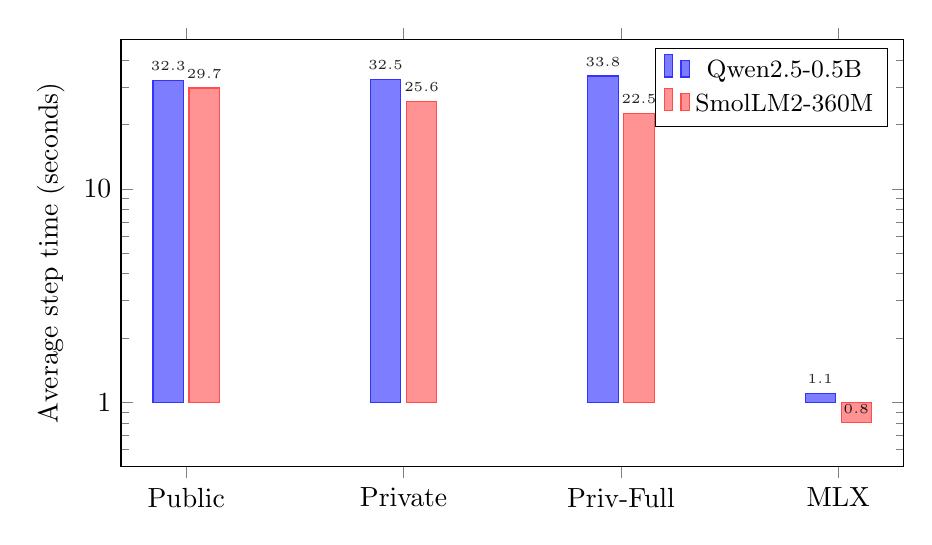
\begin{tikzpicture}
\begin{axis}[
    ybar,
    bar width=11pt,
    width=0.95\columnwidth,
    height=7cm,
    ylabel={Average step time (seconds)},
    ymode=log,
    log ticks with fixed point,
    ymin=0.5,
    ymax=50,
    symbolic x coords={Public, Private, {Priv-Full}, MLX},
    xtick=data,
    legend style={at={(0.98,0.98)}, anchor=north east, font=\small},
    every axis plot/.append style={fill opacity=0.85},
    point meta=rawy,
    nodes near coords,
    nodes near coords style={font=\tiny, /pgf/number format/fixed, /pgf/number format/precision=1},
    every node near coord/.append style={anchor=south},
]
\addplot[fill=blue!60, draw=blue!80] coordinates
    {(Public, 32.3) (Private, 32.5) ({Priv-Full}, 33.8) (MLX, 1.1)};
\addplot[fill=red!50, draw=red!70] coordinates
    {(Public, 29.7) (Private, 25.6) ({Priv-Full}, 22.5) (MLX, 0.8)};
\legend{Qwen2.5-0.5B, SmolLM2-360M}
\end{axis}
\end{tikzpicture}
\caption{Average step time across four compute paths (log scale).  MLX completes steps in 0.8--1.1~seconds versus 22--34~seconds for CPU and ANE paths.  SmolLM2 is faster than Qwen across all backends, likely due to its 3$\times$ smaller vocabulary reducing output projection cost.}
\label{fig:speed}
\end{figure}

The gap is stark.  SmolLM2-360M on MLX averages 0.8~seconds per step.  The same model on the public CPU path takes 29.7~seconds---37$\times$ slower.  Qwen2.5-0.5B shows a similar ratio: 1.1~seconds on MLX versus 32.3~seconds on public, a 29$\times$ difference.

Why is MLX so much faster?  Not because Metal GPU computes individual operations faster than the CPU.  MLX runs the entire computation graph (tokenization, forward pass, sampling, gradient computation) as a single fused pipeline on one engine.  The CPU and ANE paths serialize across engines: generate tokens on CPU or ANE, transfer data, score rewards, transfer back, compute gradients on CPU.  Each boundary adds latency.

The ANE paths don't help much with speed.  Qwen on the private path (32.5s) is essentially identical to public (32.3s).  SmolLM2 shows modest improvement: private (25.6s) is 14\% faster than public (29.7s), and private-full (22.5s) is 24\% faster.  These gains are marginal next to MLX's 37$\times$ speedup.

\textbf{Autoregressive generation is the bottleneck.}  Over 95\% of step time across every path goes to rollout generation---producing $G=4$ candidate responses of up to 128~tokens each.  This is inherently sequential.  The ANE can execute individual forward passes in under 0.2ms via the private API, but generating one response still requires 128 sequential evaluations plus KV cache management, tokenization, and sampling at each step.  Metal GPU faces the same constraint but amortizes overhead through MLX's lazy evaluation and fused kernels.

Over a full 500-step run, these differences compound.  SmolLM2 on MLX finishes in 6.7~minutes.  Qwen on MLX takes 9.2~minutes.  The same models on the public CPU path take 4.1 and 4.5~hours respectively.  A researcher can iterate on MLX hyperparameters six times in the span of a single CPU training run.

% --------------------------------------------------------------------------
% 5.3 POWER EFFICIENCY
% --------------------------------------------------------------------------
\subsection{Power Efficiency}
\label{sec:power}

Figure~\ref{fig:power} shows average system power draw.  MLX consumes the least total power despite using the Metal GPU.

\begin{figure}[t]
\centering
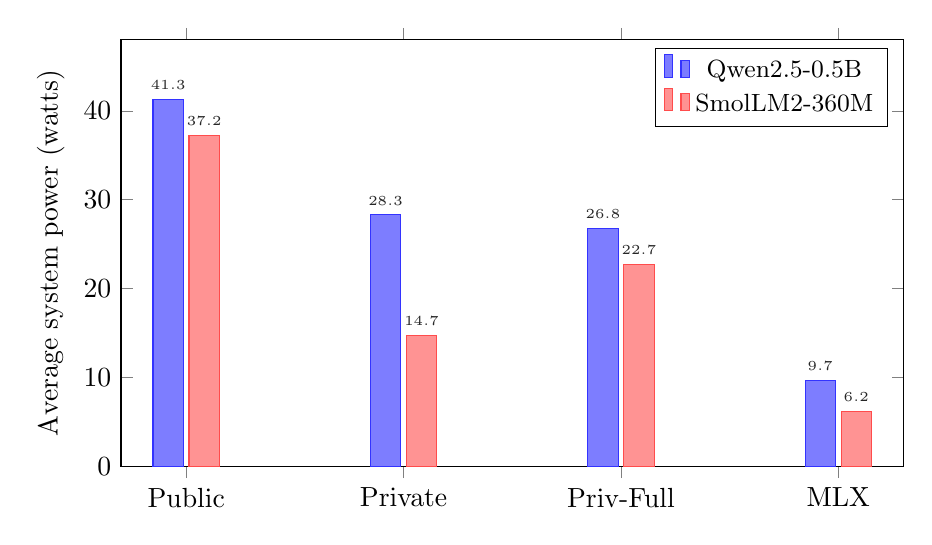
\begin{tikzpicture}
\begin{axis}[
    ybar,
    bar width=11pt,
    width=0.95\columnwidth,
    height=7cm,
    ylabel={Average system power (watts)},
    ymin=0,
    ymax=48,
    symbolic x coords={Public, Private, {Priv-Full}, MLX},
    xtick=data,
    legend style={at={(0.98,0.98)}, anchor=north east, font=\small},
    every axis plot/.append style={fill opacity=0.85},
    nodes near coords,
    nodes near coords style={font=\tiny, /pgf/number format/fixed, /pgf/number format/precision=1},
    every node near coord/.append style={anchor=south},
]
\addplot[fill=blue!60, draw=blue!80] coordinates
    {(Public, 41.3) (Private, 28.3) ({Priv-Full}, 26.8) (MLX, 9.7)};
\addplot[fill=red!50, draw=red!70] coordinates
    {(Public, 37.2) (Private, 14.7) ({Priv-Full}, 22.7) (MLX, 6.2)};
\legend{Qwen2.5-0.5B, SmolLM2-360M}
\end{axis}
\end{tikzpicture}
\caption{Average total system power across four compute paths.  CPU-only execution draws 37--41W.  ANE paths reduce draw 30--60\%.  MLX draws 6--10W because Metal GPU handles the entire workload while the CPU idles.}
\label{fig:power}
\end{figure}

The public CPU path draws the most power: 41.3W for Qwen, 37.2W for SmolLM2.  Nearly all of this is CPU utilization (GPU under~1W, ANE under~0.1W).  CPU-only training keeps all cores saturated for the entire step.

The private ANE path cuts power substantially.  SmolLM2 drops from 37.2W to 14.7W, a 60\% reduction.  Qwen's reduction is smaller: 41.3W to 28.3W (31\%).  The difference reflects model architecture.  SmolLM2's simpler attention maps more efficiently to ANE execution, offloading more work from CPU.  The private-full path shows mixed results: 26.8W for Qwen (35\% reduction) but 22.7W for SmolLM2 (39\% reduction, worse than private's 60\%).  Running backward-dx kernels on ANE adds power draw that partially offsets the forward-pass savings.

MLX dominates power efficiency for the same reason it dominates speed: Metal GPU handles the full computation graph while the CPU idles at 2--3W.  Qwen MLX draws 9.7W total (7.1W GPU).  SmolLM2 MLX draws 6.2W (4.2W GPU).

Energy per step tells the most dramatic story.  SmolLM2-360M on MLX consumes 5.0~joules per training step.  A full 500-step run uses 0.7~Wh---less than 1\% of a MacBook Pro battery.  The same model on the public path consumes 153~Wh over 500~steps.  MLX is 221$\times$ more energy efficient per step.

% --------------------------------------------------------------------------
% 5.4 LEARNING DYNAMICS
% --------------------------------------------------------------------------
\subsection{Learning Dynamics}
\label{sec:learning}

Speed and power matter only if the model actually learns.  Figure~\ref{fig:learning} shows peak-20 reward and last-50 JSON validity side by side.

\begin{figure}[t]
\centering
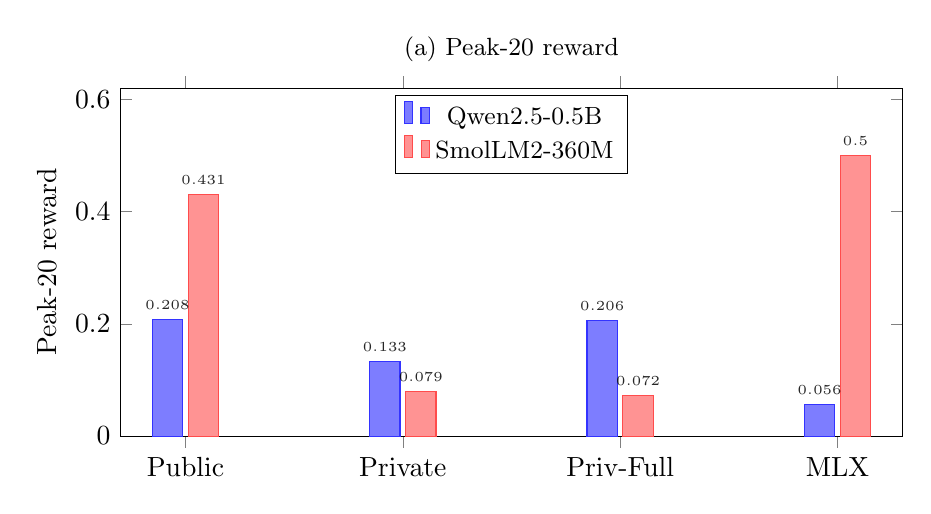
\begin{tikzpicture}
\begin{axis}[
    name=rewardplot,
    ybar,
    bar width=11pt,
    width=0.95\columnwidth,
    height=6cm,
    ylabel={Peak-20 reward},
    ymin=0,
    ymax=0.62,
    clip=false,
    symbolic x coords={Public, Private, {Priv-Full}, MLX},
    xtick=data,
    legend style={at={(0.5,0.98)}, anchor=north, font=\small},
    every axis plot/.append style={fill opacity=0.85},
    nodes near coords,
    nodes near coords style={font=\tiny, /pgf/number format/fixed, /pgf/number format/precision=3},
    every node near coord/.append style={anchor=south},
    title={\small (a) Peak-20 reward},
]
\addplot[fill=blue!60, draw=blue!80] coordinates
    {(Public, 0.208) (Private, 0.133) ({Priv-Full}, 0.206) (MLX, 0.056)};
\addplot[fill=red!50, draw=red!70] coordinates
    {(Public, 0.431) (Private, 0.079) ({Priv-Full}, 0.072) (MLX, 0.500)};
\legend{Qwen2.5-0.5B, SmolLM2-360M}
\end{axis}
\end{tikzpicture}

\vspace{0.3cm}

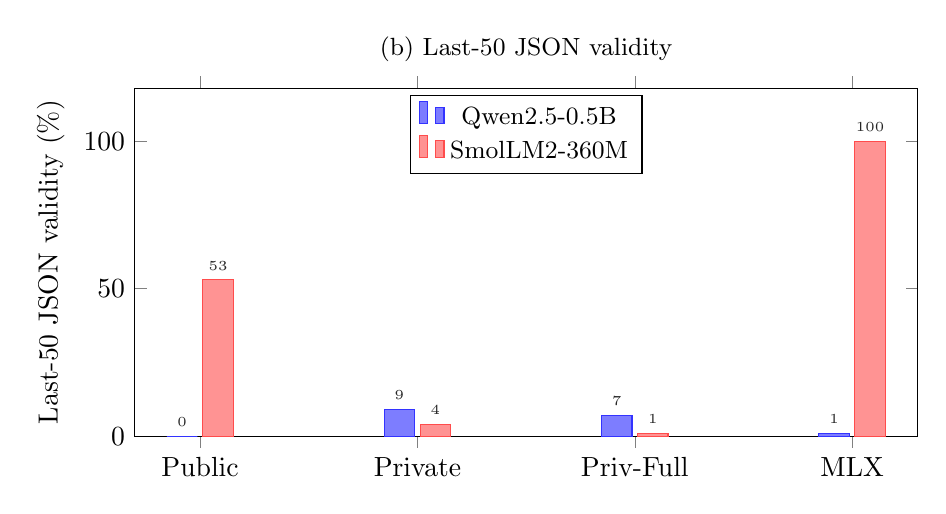
\begin{tikzpicture}
\begin{axis}[
    ybar,
    bar width=11pt,
    width=0.95\columnwidth,
    height=6cm,
    ylabel={Last-50 JSON validity (\%)},
    ymin=0,
    ymax=118,
    clip=false,
    symbolic x coords={Public, Private, {Priv-Full}, MLX},
    xtick=data,
    legend style={at={(0.5,0.98)}, anchor=north, font=\small},
    every axis plot/.append style={fill opacity=0.85},
    nodes near coords,
    nodes near coords style={font=\tiny},
    every node near coord/.append style={anchor=south},
    title={\small (b) Last-50 JSON validity},
]
\addplot[fill=blue!60, draw=blue!80] coordinates
    {(Public, 0) (Private, 9) ({Priv-Full}, 7) (MLX, 1)};
\addplot[fill=red!50, draw=red!70] coordinates
    {(Public, 53) (Private, 4) ({Priv-Full}, 1) (MLX, 100)};
\legend{Qwen2.5-0.5B, SmolLM2-360M}
\end{axis}
\end{tikzpicture}
\caption{Learning outcomes across eight experiments.  (a)~Peak-20 reward: SmolLM2 on MLX achieves the maximum possible reward (0.500).  (b)~Last-50 JSON validity: only SmolLM2 on MLX sustains 100\% validity through the end of training.}
\label{fig:learning}
\end{figure}

SmolLM2-360M on MLX is the standout result.  Peak-20 reward of 0.500 (the maximum possible) with 100\% JSON validity sustained through the final 50~steps.  This is not a handful of lucky generations.  It is a model that has genuinely learned to produce valid structured output through on-device reinforcement learning.

SmolLM2 on the public CPU path comes second.  Its peak-20 reward of 0.431 shows strong learning, and 53\% last-50 validity means it partially retains the skill.  Both paths run in fp32.  The gap between them (0.431 vs.\ 0.500, 53\% vs.\ 100\%) may reflect implementation differences: the MLX path uses Python with MLX's native LoRA, while the public path uses our custom Objective-C GRPO loop.  Alternatively, MLX's fused operations may reduce numerical drift over 500~gradient steps.  We cannot isolate the cause from these experiments alone.

The ANE paths degrade learning quality for both models.  SmolLM2 on the private path drops from 0.431 peak-20 (public, fp32) to 0.079 (private, fp16 forward).  Qwen shows the same pattern: 0.208 (public) to 0.133 (private).  Private-full fares no better.  The fp16 precision of ANE forward passes introduces noise that accumulates over 500~steps, corrupting the reward signal that drives policy updates.

Qwen2.5-0.5B never learns well on any path.  Its best result is 0.208 peak-20 reward on the public path with 0\% last-50 validity.  It picks up some learning early, then loses all JSON validity by the end of training.  On MLX, Qwen's peak-20 is just 0.056 despite MLX being the best backend for SmolLM2.  Qwen lacks the capacity for this task regardless of compute path.  Two architectural differences may explain why, despite Qwen having more parameters (490M vs.\ 362M).  Qwen's vocabulary is 3$\times$ larger (152K vs.\ 49K tokens), spreading output probability mass across more candidates and making it harder for LoRA to steer structured generation.  And SmolLM2 has more transformer layers (32 vs.\ 24), which means more LoRA intervention points even though each layer is smaller.

Consider what this means.  SmolLM2 at 362M parameters learns perfectly on MLX.  Qwen at 490M parameters, 35\% larger, fails on every compute path.  Parameter count does not predict on-device learning success.  The capacity threshold from Paper~II~\cite{maloney2025capacity} manifests here as a property of architecture interacting with task requirements, not raw size.

% ============================================================================
% 6. DISCUSSION
% ============================================================================
\section{Discussion}
\label{sec:discussion}

\subsection{Why MLX Dominates}

We spent months building CoreML pipelines, writing Objective-C GRPO loops, implementing private API bootstraps, and hand-coding backward-dx kernels for the ANE.  We expected the Neural Engine's power efficiency to make it the preferred engine for rollout generation, with Metal GPU handling only gradients.  The data says we were wrong.

The primary advantage is architectural: MLX runs the entire computation graph on a single engine with no serialization boundaries.  The CPU and ANE paths move data between engines at every phase of the training loop---generate tokens on CPU or ANE, transfer to CPU for scoring, compute gradients on CPU, optionally synchronize weights back to ANE.  MLX eliminates all transfers.  On top of that, MLX's lazy evaluation and operation fusion reduce per-token overhead during autoregressive generation.  Individual ANE forward passes take under 0.2ms, but the Objective-C orchestration between passes (tokenization, sampling, KV cache update, next-token preparation) adds overhead that compounds over 128~tokens $\times$ 4~rollouts $\times$ 500~steps.  The power story reinforces this: Metal GPU at 4--7W turns out to be more efficient than saturating the CPU at 37--41W for sustained matrix operations.  We did not expect that going in.

\subsection{The Precision Tax}

ANE paths run forward passes in fp16.  This has a measurable cost.

SmolLM2 on the public path (fp32 throughout) achieves 0.431 peak-20 reward.  The same model on the private path (fp16 forward, fp32 backward) drops to 0.079.  The most salient difference is forward-pass precision, though the two paths also differ in runtime implementation and engine serialization.  Our leading explanation: over 500~steps with $G=4$ rollouts each, fp16 rounding errors in the policy log-probabilities accumulate.  The advantage estimates computed from noisy log-probs push the policy in slightly wrong directions, and those errors compound step after step.  We cannot fully rule out contributions from the runtime differences, but precision is the most likely driver given the magnitude of the gap.

This finding has implications beyond Apple Silicon.  Any system that uses reduced-precision inference for GRPO rollouts while computing gradients in full precision should expect degraded learning.  The precision boundary between inference and training is not free.

\subsection{When ANE Matters}

Our results might suggest the ANE is useless for on-device ML.  That conclusion would be too strong.

The ANE reduces system power by 30--60\% compared to CPU-only execution.  For inference-only deployment, where an agent serves predictions without training, this is significant.  An agent running continuous inference at 3W on battery operates 10$\times$ longer than one running at 30W on Metal GPU.  Paper~V~\cite{maloney2025moe} identified power efficiency as a deployment constraint.  The ANE addresses it for inference workloads.

For training, the ANE's limitation is precision and serialization, not power.  If Apple were to support fp32 on the Neural Engine, or if CoreML exposed a native backward-pass API, the ANE could potentially match MLX's learning quality at lower power.  Neither capability exists today.

\subsection{The Autoregressive Bottleneck}

Across all eight experiments, rollout generation consumes over 95\% of step time.  Gradient computation is fast.  Reward scoring is trivial.  The bottleneck is generating 4~candidate responses of up to 128~tokens each, one token at a time, regardless of which engine does the work.

This carries a practical implication: optimizing gradient computation has almost no impact on on-device GRPO throughput.  The private-full path routes backward-dx kernels to the ANE, saving CPU cycles during backpropagation.  The time savings are invisible because backward passes account for less than 5\% of step time.

Speculative decoding, parallel generation across rollouts, or shorter response budgets would have more impact on training throughput than any improvement to gradient computation.  Future work on on-device RL should focus on rollout acceleration.

\subsection{Series Implications}

The capacity threshold from Paper~II~\cite{maloney2025capacity} manifests here, but differently than on server hardware.  On datacenter GPUs, the threshold is primarily about model size: below 1B parameters, models lose JSON validity during GRPO training and never recover.  On-device, the threshold interacts with architecture and precision.

Qwen2.5-0.5B (490M) fails to sustain JSON validity on any compute path.  SmolLM2-360M (362M) succeeds perfectly on MLX despite having fewer parameters.  The combination of vocabulary size (49K vs.~152K), attention design, and training precision matters more than raw parameter count in the constrained on-device setting.

Paper~IV~\cite{maloney2025dynamics} found that early reward trajectories predict final outcomes on server hardware.  The same holds here.  If a model hasn't shown meaningful reward by step~50, it won't start at step~300.  SmolLM2 on MLX and the public path both show strong early signals and sustain learning through 500~steps.  Every other configuration shows weak early rewards and never recovers.  This makes on-device experimentation practical: with MLX completing a step in under a second, you can evaluate whether a configuration will work within the first minute of training.

\subsection{Limitations}

This study has several constraints that bound how far the results generalize.

Each of the eight experiments ran once.  We report no variance estimates, no confidence intervals, and no seed sweeps.  The headline numbers---0.500 peak-20 reward, 100\% last-50 validity for SmolLM2 on MLX---are single-run observations.  They are directional, not definitive.  GRPO training is stochastic; a different random seed could produce meaningfully different reward trajectories, particularly for configurations near the boundary of learning (SmolLM2 on the public path at 53\% validity, for instance).  The immediate next step is to run 3~seeds per cell across all 24~experiments and report means with standard deviations.

We tested two models, both under 500M parameters.  Two data points cannot cleanly separate architecture effects from backend effects.  The observation that SmolLM2-360M outperforms the larger Qwen2.5-0.5B is suggestive---vocabulary size, layer count, and attention design all differ---but we cannot attribute the gap to any single factor.  Adding 2--3 models in the 1B--3B range on MLX would strengthen the architectural claims considerably.

All experiments ran on a single machine (MacBook Pro, M-series, 36GB).  We do not know how results transfer to other M-series chips with different core counts, memory bandwidth, or thermal envelopes.  The ANE precision behavior may also differ across chip generations.

Finally, the CLINC intent classification task is a single, relatively constrained structured-output problem.  We have not tested whether these findings hold for longer-form generation, multi-turn dialogue, or tasks that require reasoning chains.

% ============================================================================
% 7. CONCLUSION
% ============================================================================
\section{Conclusion}
\label{sec:conclusion}

We compared four compute paths for on-device GRPO training on Apple Silicon, running 500-step experiments across eight configurations.

MLX on Metal GPU is the clear winner: 30--40$\times$ faster, 4--6$\times$ lower power, over 200$\times$ more energy efficient than CPU-based training.  SmolLM2-360M on MLX achieves 100\% JSON validity with maximum reward in under seven minutes on a single laptop charge.  On-device reinforcement learning is not just viable.  For the right model on the right backend, it works perfectly.

The Apple Neural Engine reduces power consumption for inference but introduces an fp16 precision cost that degrades training.  CPU-based training in fp32 produces better learning outcomes than ANE-based training in fp16.  And autoregressive rollout generation, not gradient computation, is the binding constraint across all paths.

Specialization is not the answer.  Simplicity is.  One engine, full precision, no serialization boundaries.

% ============================================================================
% APPENDIX
% ============================================================================
\appendix

\section{Training Hyperparameters}
\label{app:hyperparams}

Table~\ref{tab:hyperparams} lists the hyperparameters used across all eight experiments.  All settings are identical across compute paths.

\begin{table}[ht]
\centering
\caption{Training hyperparameters (identical across all experiments).}
\label{tab:hyperparams}
\begin{tabular}{lc}
\toprule
\textbf{Parameter} & \textbf{Value} \\
\midrule
Training steps & 500 \\
Group size ($G$) & 4 \\
Learning rate & $5 \times 10^{-6}$ \\
LoRA rank & 4 \\
LoRA layers & 4 (attention projections) \\
KL penalty ($\beta$) & 0.1 \\
Max generation tokens & 128 \\
Gradient clip norm & 1.0 \\
Optimizer & AdamW \\
$\beta_1, \beta_2$ & 0.9, 0.999 \\
Weight decay & 0.01 \\
\bottomrule
\end{tabular}
\end{table}

\section{CoreML Conversion Notes}
\label{app:coreml}

Both Qwen2.5-0.5B and SmolLM2-360M required operation-level rewrites to compile for ANE execution via \texttt{coremltools}~\cite{apple2023coremltools}.  Four classes of issues arose:

\begin{itemize}[leftmargin=*]
\item \textbf{Embedding gather:}  The ANE does not support \texttt{gather} for embedding lookups.  We pre-compute embeddings on CPU and pass them as input tensors to the CoreML model.

\item \textbf{GQA head expansion:}  Qwen2.5 uses grouped-query attention with \texttt{repeat\_interleave} for key-value head expansion.  This operation is unsupported on ANE.  We replace it with an \texttt{unsqueeze}$\,\to\,$\texttt{expand}$\,\to\,$\texttt{reshape} sequence that produces identical results.

\item \textbf{Dimension padding:}  ANE requires tensor dimensions to be multiples of~32.  We pad trailing dimensions with zeros and slice results after computation.

\item \textbf{Tensor layout transposition:}  The ANE uses channel-major layout (\texttt{[1, C, 1, S]}) while CPU uses row-major (\texttt{[S, C]}).  Every CPU$\leftrightarrow$ANE data transfer requires explicit transposition: \texttt{input[t*dim+c]} $\to$ \texttt{ptr[c*seq+t]}.  Raw \texttt{memcpy} between layouts produces garbage outputs.
\end{itemize}

KV cache management uses CoreML state tensors with \texttt{register\_buffer()} in the PyTorch wrapper.  The \texttt{name} attribute must be set on \texttt{StateType}, not on \texttt{TensorType}.

We trace only the $S=1$ decode path, since GRPO rollouts are autoregressive.  The prefill path ($S>1$) triggers conditional branches in the attention mechanism that \texttt{coremltools} cannot trace through.

\section{Backward-dx Kernel Implementation}
\label{app:backward}

The private-full path computes input gradients (backward dx) on the ANE.  We originally attempted this through the private bootstrap API (\texttt{\_ANEInMemoryModel}), which worked for small test models but crashed at Qwen and SmolLM2 scale with \texttt{ANEProgramProcessRequestDirect() Failed}.

The working implementation uses CoreML's public API.  We compile a separate CoreML model that computes the Jacobian-vector product for each layer, targeting ANE compute units.  The Objective-C runtime (\texttt{coreml\_eval\_backward} in \texttt{coreml\_runtime.\{h,m\}}) orchestrates the backward pass by chaining per-layer evaluations.

% ============================================================================
% BIBLIOGRAPHY
% ============================================================================
\bibliographystyle{plainnat}
\bibliography{refs}

\end{document}
